\section{Evaluation on retrieval systems}

The goal of evaluation is to assess the quality of the results 
obtained by an IR system.
There's the need of knowing a \emph{ground truth}, so an annotated corpus 
where for each task we know what documents are relevant. The annotations
could be created manually or derived from the data, if it contains 
annotations.

\subsection{The notion of quality}
Given a corpus $C$ and a query $q$, the task is to find a set of 
documents $A_{q,C}$ that match $q$, but after retrieving such documents, 
there's the need to estimate the quality of results.

\paragraph{Precision}
To formalise the quality of the retrieved documents $A_{q,C}$ we could 
count how many of these documents are relevant to $q$, this 
is the notion of precision:
$$\mathit{Prec} = \frac{\mathit{relevant\;retrieved}}{\mathit{retrieved}}$$
Note that in order to know if a document is relevant or not we need the 
ground truth or a user feedback.

This measure does not suffice, as for instance, if we retrieve 
only one correct document we would have maximum precision.

\paragraph{Recall}
The precision measure does not take in consideration how many relevant 
documents are there, that is crucial to assess quality of a query result.
So we can consider another measure, called Recall:
$$\mathit{Rec} = \frac{\mathit{relevan\;retrieved}}{\mathit{relevant}}$$

\paragraph{Information need}
Given the two quality measures, should we aim at better precision or more 
recall? Trivially both, but it actually depends on the information need.\\
In some cases a really high recall is not necessary, while other times
a lower precision could be accepted while not missing anything relevant.

\paragraph{F1 Score}
To take into consideration both precision and recall, we could take 
a weighted mean, so a tradeoff between the twos 
$$\mathit{F1} = \frac{2\cdot\mathit{Prec}\cdot\mathit{Rec}}
{\mathit{Prec} + \mathit{Rec}}$$

\paragraph{Baseline system}
To assess the quality of an IR system, we need a baseline system, 
something trivial such as tossing a coin to decide whereas a document 
is relevant or not. 
Given its quality measure, we can infer the quality of our, hopefully, 
more complex system, in fact, quality measures can't be seen as absolute 
values, there's always the need to compare.

\subsection{Quality measures}
To formally define the notions introduced in the previous section, we need
to take into consideration a more detail measure for errors.

\paragraph{Confusion Matrix}
Given a query $q$, a ground truth $E_q$ of relevant documents with respect 
to $q$, and a set of retrieved documents $A_q$, we define this matrix:
\begin{center}
    \begin{tabular}{c | c |c}
            & $d \in E_q$ & $d \notin E_q$\\
            \hline
            $d \in A_q$ & True positive & False positive\\
            \hline
            $d \notin A_q$ & False Negative & True Negative\\
    \end{tabular}
\end{center}
So now we can redefine the \emph{precision}, \emph{recall} and \emph{F1} 
measures as follows
$$\mathit{Prec} = \frac{\mathit{TP}}{\mathit{TP} + \mathit{FP}}\;\;\;
\mathit{Rec} = \frac{\mathit{TP}}{\mathit{TP} + \mathit{FN}}\;\;\;
\mathit{F1} = \frac{\mathit{TP}}{\mathit{TP} + \frac{1}{2}(\mathit{FP} + \mathit{FN})}$$
The actual confusion matrix is obtained by counting the documents given the retrieved 
ones and the ground truth. 

The matrix can be useful to estimate the system parameters, for instance, 
if the number of retrieved documents is set to a certain value $k$ and 
the value of true positives is really high, probably a smaller $k$ would do the job, 
while if a lot positives are left out, i.e, the matrix has a high number of
false negatives, maybe an higher $k$ would make the system better.

\paragraph{Other measures}
The are a lot of measures to estimate the quality of a system, such as 
\emph{specificity}, \emph{negative predictive value}, \emph{miss-rate}, 
\emph{fall-out} and \emph{accuracy}. 
Finding the right measure is really important, for instance, using accuracy with
an unbalanced dataset is not better than precision, recall and F1.

\subsection{Evaluation of ranking systems}
We talked about boolean retrieval systems and we took into consideration 
if a document is retrieved or not.

In a raking scenario, we want to give importance not only to precision and recall, 
but also to the rank assigned by the system.

\paragraph{Setting a threshold}
One way to go is to set a specific threshold and compute the precision and recall 
of those top documents.
This method does not take into consideration the ranking of the documents.

\paragraph{Precision at K}
If we take the first $K$ retrieved documents, ordered by rank, we can estimate 
the quality of the rank by computing the precision for the top $K$ documents.
By iterating the threshold we can better estimate the performances, opposed to 
setting a unique threshold.\\
To decide what thresholds to use we could use the distribution of the system ranking.

\paragraph{Discounted cumulative gain}
This approach takes into consideration the ranking and discount the gain given by
a document with respect to its position in it.
$$\mathit{DCG} = \sum_{i = 1}^n\frac{R_j}{\log(i+1)}$$
where $R_j$ is the rank assigned to a document.

\paragraph{Precision vs Recall curve}
Another approach is to compute precision and recall measures at each point in the ranking.
If we take the measurements and plot them, we find a correlation between precision 
and recall and if we compute the integral of that function, we obtain the average precision.

To have a smoother curve, it's possible to interpolate the precision, so for each 
point in the recall axis, we take the maximum precision of consecutive points.

\begin{figure}[h]
    \centering
    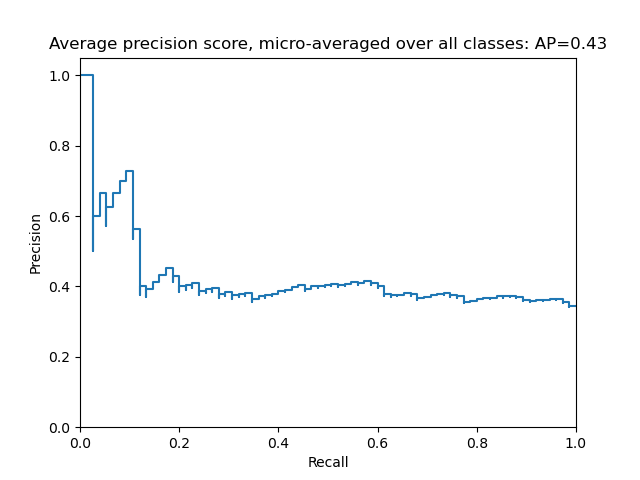
\includegraphics[width=0.7\textwidth]{images/precision-recall.png}
    \caption{Example of a non-interpolated precision and recall curve}
\end{figure}